\label{appendices}

\renewcommand{\thechapter}{A}
%\chapter{Commands used to run NOBLE Coder}
%\label{app:commands_run_noble}
%
%\begin{lstlisting}[language=bash]
%$ java -jar NobleCoder-1.0.jar -terminology radlex \
%-input [portuguese reports path] -output [output path] \
%-search all-match\textit{
%
%$ java -jar NobleCoder-1.0.jar -terminology radlex \
%-input [portuguese reports path] -output [output path] \
%-search best-match
%\end{lstlisting}
%
%\chapter{Uploading RadLex ontology to NOBLE}
%\label{app:change_radlex_noble}
%
%I had to edit the RadLex ontology .owl file before it could be correctly processed and %uploaded to NOBLE Coder. In the original .owl file the properties  "Preferred\_name" and %"Synonym" are considered to be \textit{DatatypeProperty} but I had to change both to %\textit{AnnotationProperty}. That is, where in the file was
%
%\begin{lstlisting}[language=xml]
%<owl:DatatypeProperty rdf:ID="Preferred_name">
%</owl:DatatypeProperty>
%\end{lstlisting}
%
%I have had to change it to:
%
%\begin{lstlisting}[la	nguage=xml]
%<owl:AnnotationProperty rdf:ID="Preferred_name">
%</owl:AnnotationProperty>
%\end{lstlisting}
%
%And the analogous thing for the "Synonym" property.


\chapter{Macro Evaluations}
\label{app:macro_evaluations}

\begin{figure}[ht]
	\centering
	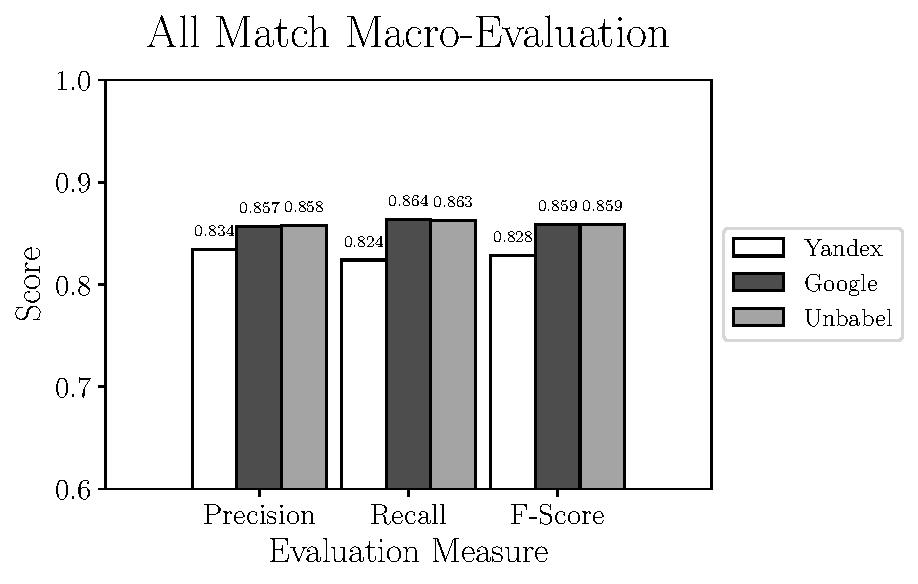
\includegraphics[width=0.9\textwidth]{SupportFiles/plots/all_match_macro_total_plot.pdf}
	\caption{Macro Evaluation of Translations being tested (All Match)}
	\label{app:macro_eval_all}
\end{figure}

\begin{figure}[ht]
	\centering
	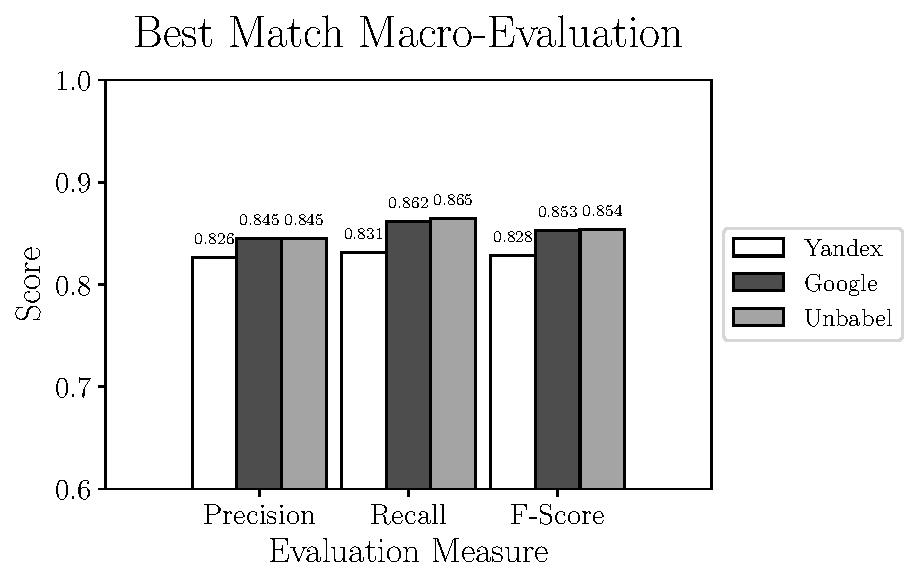
\includegraphics[width=0.9\textwidth]{SupportFiles/plots/best_match_macro_total_plot.pdf}
	\caption{Macro Evaluation of Translations being tested (Best Match)}
	\label{app:macro_eval_best}
\end{figure}

\begin{figure}[ht]
	\centering
	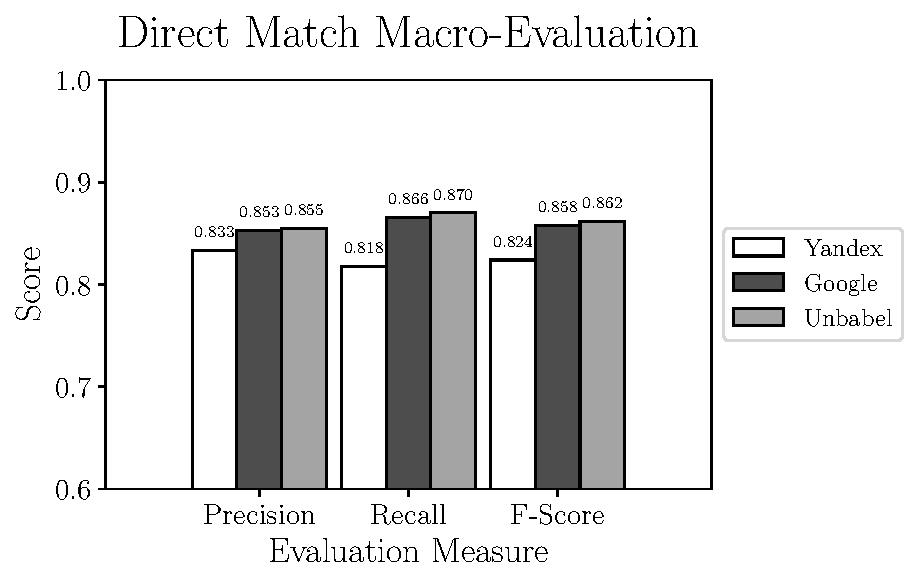
\includegraphics[width=0.9\textwidth]{SupportFiles/plots/direct_match_macro_total_plot.pdf}
	\caption{Macro Evaluation of Translations being tested (Direct Match)}
	\label{app:macro_eval_direct}
\end{figure}


\begin{figure}[ht]
	\centering
	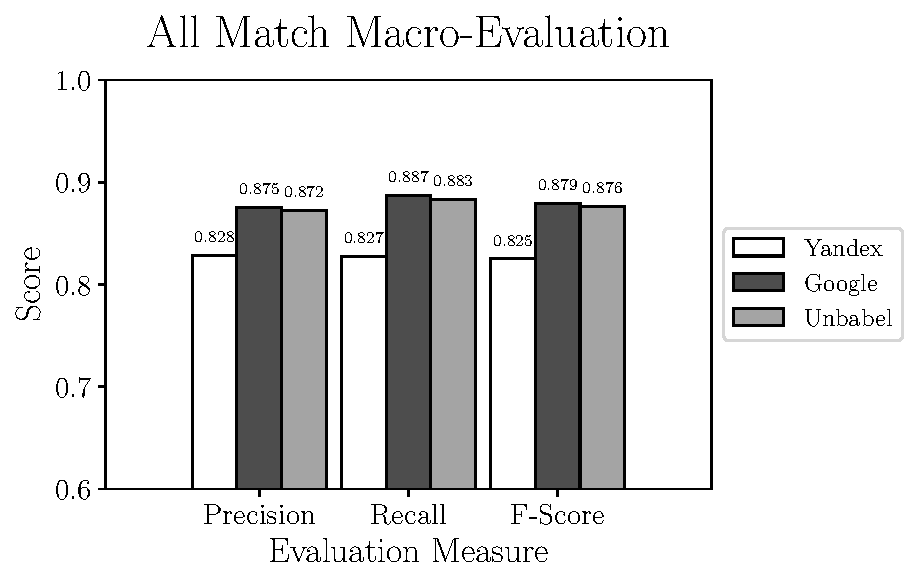
\includegraphics[width=0.9\textwidth]{SupportFiles/plots/all_match_macro_clinical_anatomical_subtrees_plot.pdf}
	\caption{Macro Evaluation of translations being tested, considering just the terms from RadLex \textit{clinical finding} and \textit{anatomical entity} subtrees (All Match)}
	\label{app:macro_eval_subtrees_all}
\end{figure}


\begin{figure}[ht]
	\centering
	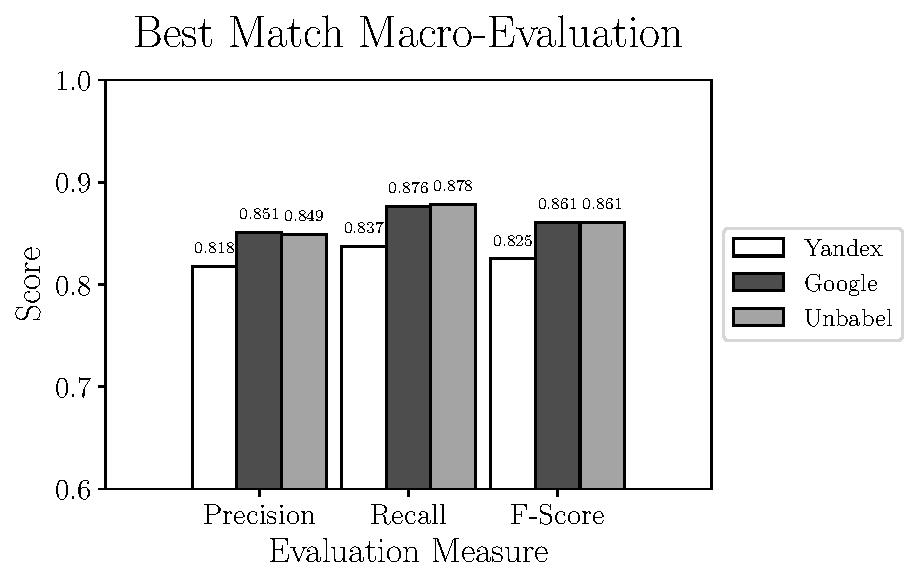
\includegraphics[width=0.9\textwidth]{SupportFiles/plots/best_match_macro_clinical_anatomical_subtrees_plot.pdf}
	\caption{Macro Evaluation of translations being tested, considering just the terms from RadLex \textit{clinical finding} and \textit{anatomical entity} subtrees (Best Match)}
	\label{app:macro_eval_subtrees_best}
\end{figure}


\begin{figure}[ht]
	\centering
	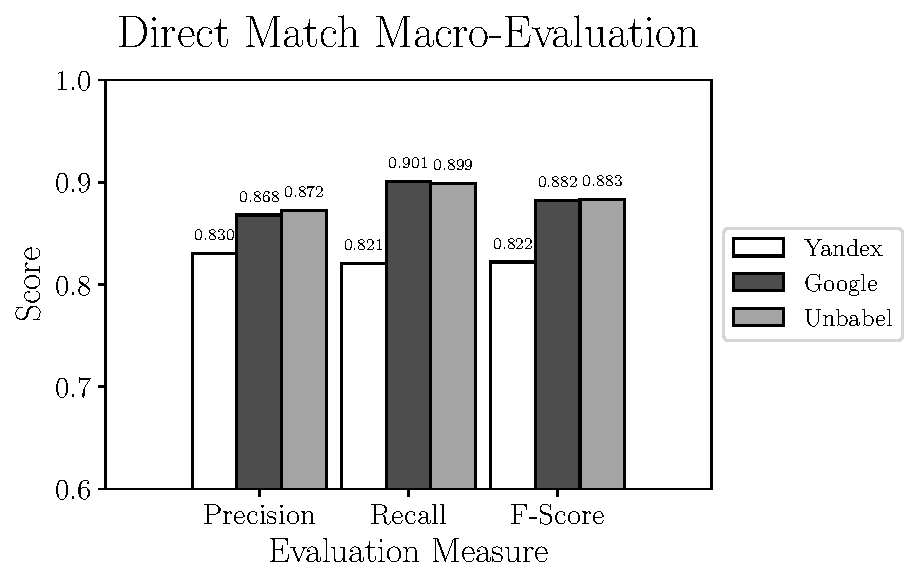
\includegraphics[width=0.9\textwidth]{SupportFiles/plots/direct_match_macro_clinical_anatomical_subtrees_plot.pdf}
	\caption{Macro Evaluation of translations being tested, considering just the terms from RadLex \textit{clinical finding} and \textit{anatomical entity} subtrees (Direct Match)}
	\label{app:macro_eval_subtrees_direct}
\end{figure}



\chapter{Subtrees Analysis}
\begin{table}[ht]
	\centering
	\caption{Number of RadLex \textit{clinical finding} or \textit{anatomical entity} terms found by document}
	\begin{tabular}{lrrr}
		\toprule
		\textbf{Translation}   &   \textbf{Direct Match} &   \textbf{All Match} &   \textbf{Best Match} \\
		\midrule
		\textbf{Human}         &         36.82	  &  54.76	 &    41.20 \\
		\textbf{Yandex}        &         35.25	  &  53.33	  &   41.75 \\
		\textbf{Google}        &         37.73	  &  55.55	  &   42.35 \\
		\textbf{Unbabel}       &         37.59	 &   55.14	 &    42.45 \\
		\bottomrule
	\end{tabular} 
	\label{app:terms_by_document_subtrees}
\end{table}

\chapter{Error Evaluations}
\begin{table}[ht]	
	\centering
	\caption{Number of Errors Belonging to Each Category, by Translation Type. The column "?" contains the count of the errors for which I could not attribute a category}
	\begin{tabular}{lrrrr}
		\toprule
		\textbf{Translation}   &   \textbf{Wrong Translation} &   \textbf{Not Wrong Translation} &   \textbf{?} & \textbf{Total} \\
		\midrule
			\textbf{Human}         &         25 &  71 &  4 &   100 \\
			\textbf{Yandex}        &         19 &  64 &  3 &   86 \\
			\textbf{Google}        &         18 &  64 &  3 &   85 \\
			\textbf{Unbabel}       &         62 &  199 & 10 &  271 \\
		\bottomrule
	\end{tabular} 
	\label{app:error_analysys_error_by_category}
\end{table}

%\begin{table}[ht]   
%    \centering
%    \caption{Number of Errors belonging to each Subcategory of the Wrong Translation Category, by Translation Type}
%    \begin{tabular}{lrrrrrrrrrr}
%        \toprule
%            \textbf{Translation}   &   \textbf{General} &  \textbf{Extra word} &  \textbf{Did not translate original} &   \textbf{Hyphen} &  \textbf{Didn’t translate initials} &   %\textbf{Word Missing} &    \textbf{MT is not specific enough} &   \textbf{Different lexical variation} & \textbf{Not the most correct term} &   \textbf{Total} \\
%        \midrule
%            \textbf{Yandex}        &         13 & 1 & 6 & 2 & 1 & 2 & 0 & 0 & 0 & 25 \\
%            \textbf{Google}        &         10 & 1 & 0 & 0 & 2 & 2 & 2 & 1 & 1 & 19 \\
%            \textbf{Unbabel}       &         12 & 1 & 0 & 0 & 0 & 1 & 2 & 0 & 2 & 18 \\
%        \bottomrule
%    \end{tabular} 
%    \label{app:error_analysys_error_by_subcategory}
%\end{table}


